\documentclass{beamer}
\usetheme{Berlin}

\usepackage[UTF8, fontset=fandol]{ctex}
\usepackage{hyperref}
\usepackage{latexsym,xcolor,multicol,booktabs,calligra}
\usepackage{amsmath,amssymb,BOONDOX-cal,bm}
\usepackage{graphicx,stackengine}
\usepackage{algorithm}
\usepackage{algorithmic}



%-----------------------------------------------------
% Metadata
%-----------------------------------------------------
\author{Dr RP @ IIIT Sri City}
\title{Personalized Federated Contrastive Learning for Recommendation}
\subtitle{Presentation based on FedPCL paper}
\institute{IIIT Sri City — Group Project}
\date{14 Feburary 2026}
% Note: Ensure the logo file exists or remove this line
\logo{
\includegraphics[height=0.8cm]{iiits-logo-small.png}\hspace*{0.3cm}}

\begin{document}

% Slide 1
\begin{frame}
  \titlepage
\end{frame}

% Slide 2
\begin{frame}{Outline}
  \tableofcontents[sectionstyle=show,subsectionstyle=show/shaded/hide]
\end{frame}

%-----------------------------------------------------
\section{Introduction}
% Slide 3
\begin{frame}{Introduction}
  \begin{itemize}
    \item This work proposes \textbf{FedPCL}: a federated, GNN-based recommendation framework that (1) uses \emph{structural contrastive learning} to mitigate data sparsity and (2) provides \emph{personalized models} via cluster-level + global aggregation.
    \item Key problems addressed: \textbf{data sparsity} in client-local data and \textbf{non-IID heterogeneity} across users.
    \item High-level approach: structural neighbors in GNN $\Rightarrow$ contrastive loss; server-side clustering $\Rightarrow$ cluster models + global model $\Rightarrow$ weighted combination per client.
  \end{itemize}
\end{frame}

%-----------------------------------------------------
\section{Motivation}
% Slide 4
\begin{frame}{Motivation}
\small
\begin{itemize}
  \item Traditional \textbf{centralized recommender systems} require collecting user interaction data on a server, which raises serious \textbf{privacy, security, and regulatory concerns} (e.g., GDPR).
  
  \item \textbf{Federated learning (FL)} addresses privacy by keeping user data on local devices and only sharing model updates; however, this setting introduces new challenges for recommendation.

  \item First, each client observes only a \textbf{small and sparse subset} of interactions, making it difficult to learn high-quality user and item embeddings, especially for GNN-based models.

  \item Second, user preferences across clients are \textbf{highly heterogeneous (non-IID)}, so a single globally averaged model (e.g., FedAvg) fails to capture personalized interests and often degrades recommendation performance.
\end{itemize}
\end{frame}


%-----------------------------------------------------
% Slide 5
\begin{frame}{Team contributions}
  \textbf{Team members (3):}
  \begin{itemize}
    \item \textbf{Anish Mahapatra} — studied \textbf{MovieLens-100K} dataset; assisted with model formulation, experiments and BPR training.
    \item \textbf{Saumya Suman} — studied \textbf{Steam-200K} dataset; implemented data preprocessing, experiments and visualization.
    \item \textbf{Mithil Patidar} — studied \textbf{FilmTrust} dataset; performed ablation studies and evaluation pipelines.
  \end{itemize}
  \vspace{4pt}
  \textbf{Shared work:} analysis, algorithm mathematical write-up, implementing FedPCL variants, compiling results and writing the report.
\end{frame}

%-----------------------------------------------------
% Slide 6
\begin{frame}{Contributions (from the paper)}
  \begin{enumerate}
    \item Propose \textbf{FedPCL}: personalized FL framework that combines structural contrastive learning with multicenter aggregation.
    \item Design \textbf{structure-aware contrastive objective} leveraging GNN layer outputs (structural neighbors).
    \item Propose \textbf{cluster-level + global model aggregation} to form personalized models for each client.
    \item Extensive experiments on five datasets showing consistent performance gains vs baselines.
  \end{enumerate}
\end{frame}

%-----------------------------------------------------
\section{Related Work}
% Slide 7.1
\begin{frame}{Related Work: GNNs for Recommendation}

\begin{columns}[T] % T = top aligned
  %---------------- LEFT COLUMN ----------------
  \begin{column}{0.58\textwidth}
    \begin{itemize}
      \item User–item interactions naturally form a \textbf{bipartite graph}.
      \item \textbf{Graph Neural Networks (GNNs)} propagate information through neighbors to capture higher-order relationships.
      \item \textbf{LightGCN (He et al., SIGIR 2020)} simplifies GCNs by removing feature transformation and nonlinearities.
      \item GNN-based models significantly outperform MF-based methods in sparse recommendation settings.
    \end{itemize}
  \end{column}

  %---------------- RIGHT COLUMN ----------------
  \begin{column}{0.40\textwidth}
    \centering
    
\includegraphics[width=\linewidth]{gnn_recommendation.png}
  \end{column}
\end{columns}

\end{frame}

%Slide 7.2
\begin{frame}{Related Work: Contrastive Learning}

\begin{columns}[T]
  %---------------- LEFT COLUMN ----------------
  \begin{column}{0.58\textwidth}
    \begin{itemize}
      \item \textbf{Contrastive Learning (CL)} is a self-supervised learning paradigm.
      \item It maximizes agreement between \textbf{positive pairs} and minimizes similarity with \textbf{negative pairs}.
      \item \textbf{InfoNCE loss} is widely used in vision, NLP, and graph representation learning.
      \item In recommender systems, CL improves embedding quality and alleviates \textbf{data sparsity}.
    \end{itemize}
  \end{column}

  %---------------- RIGHT COLUMN ----------------
  \begin{column}{0.40\textwidth}
    \centering
    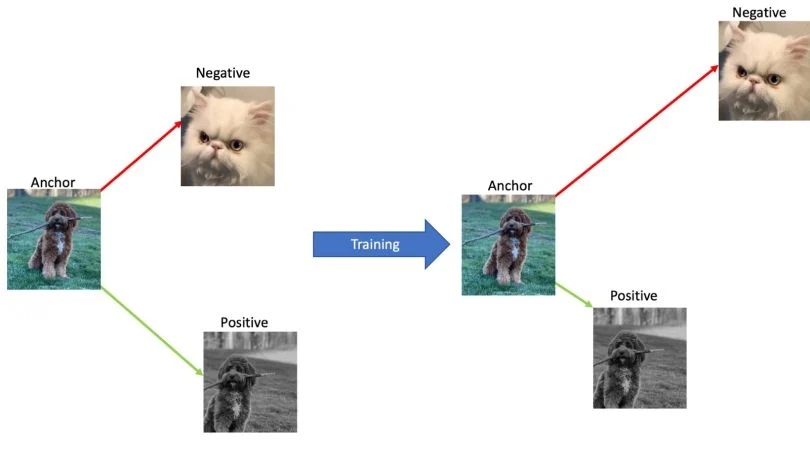
\includegraphics[width=\linewidth]{contrastive_learning_graph.png}
  \end{column}
\end{columns}

\end{frame}

%Slide 7.3
\begin{frame}{Related Work: Federated Recommendation}

\begin{columns}[T]
  %---------------- LEFT COLUMN ----------------
  \begin{column}{0.58\textwidth}
    \begin{itemize}
      \item \textbf{Federated Learning (FL)} enables collaborative training without sharing raw user data.
      \item \textbf{FedAvg (McMahan et al., 2017)} aggregates local models but assumes IID data.
      \item Extensions such as \textbf{FedMF}, \textbf{FedGNN}, and \textbf{PerFedRec (2022)} introduce privacy and personalization.
      \item Key challenges remain: \textbf{non-IID data} and \textbf{data sparsity}.
      \item \textbf{FedPCL} jointly addresses these via GNNs, contrastive learning, and personalized aggregation.
    \end{itemize}
  \end{column}

  %---------------- RIGHT COLUMN ----------------
  \begin{column}{0.40\textwidth}
    \centering
    
\includegraphics[width=\linewidth]{federated_recommendation.png}
  \end{column}
\end{columns}

\end{frame}


%-----------------------------------------------------
% Slide 8
\begin{frame}{Methodology — Overview}
  \begin{itemize}
    \item \textbf{Client side:}
      \begin{itemize}
        \item Local GNN on user--item subgraph $\Rightarrow$ multi-layer embeddings.
        \item Structural neighbor contrastive loss (InfoNCE-style) using even-layer outputs as positive samples (homogeneous neighbors).
        \item BPR ranking loss for implicit feedback.
        \item LDP (add noise) applied to gradients before upload.
      \end{itemize}
    \item \textbf{Server side:}
      \begin{itemize}
        \item Cluster user embeddings (K-means) into $K$ groups.
        \item Compute cluster-level models (FedAvg within cluster) and global model (average cluster models).
        \item Send cluster + global model to clients; clients combine them using weights for personalization.
      \end{itemize}
  \end{itemize}
\end{frame}

%-----------------------------------------------------
\section{Key Equations}
% Slide 9
\begin{frame}{Key equations (I)}
  \begin{block}{BPR ranking loss}
    \[
      \mathcal{L}_{\text{BPR}} = - \sum_{(u,i,j)\in \mathcal{D}} \ln \sigma(\hat r_{ui} - \hat r_{uj})
    \]
    where $\hat r_{ui}=f(e_u,e_i)$ (dot-product used in experiments).
  \end{block}
  \begin{block}{Structure-contrastive (InfoNCE) — users}
    \[
    \mathcal{L}_{\text{Con}}^{U} = -\sum_{i\in U}\log \frac{\exp\big(e_i^{(l)}\cdot e_i^{(0)}/\tau\big)}
    {\sum_{j\in U}\exp\big(e_i^{(l)}\cdot e_j^{(0)}/\tau\big)}
    \]
    where $e^{(l)}$ is the GNN output at even layer $l$ (structural neighbor embedding), $e^{(0)}$ initial embedding.
  \end{block}
\end{frame}

% Slide 10
\begin{frame}{Key equations (II)}
  \begin{block}{Items contrastive loss (analogous)}
    \[
    \mathcal{L}_{\text{Con}}^{V} = -\sum_{v\in V}\log \frac{\exp\big(e_v^{(l)}\cdot e_v^{(0)}/\tau\big)}
    {\sum_{n\in V}\exp\big(e_v^{(l)}\cdot e_n^{(0)}/\tau\big)}
    \]
  \end{block}
  \begin{block}{Full client loss}
    \[
      \mathcal{L} = \mathcal{L}_{\text{BPR}} + \beta_1\big(\mathcal{L}_{\text{Con}}^{U} + \lambda \,\mathcal{L}_{\text{Con}}^{V}\big) + \beta_2\|\Theta\|_2^2
    \]
  \end{block}
  \begin{block}{Personalized model composition}
    \[
      h_u^{(t)} = \mu_1 h_{C(u)}^{(t)} + \mu_2 h_{\text{global}}^{(t)}
    \]
  \end{block}
\end{frame}

%-----------------------------------------------------
% Slide 11
\begin{frame}{LDP and aggregation}
  \begin{itemize}
    \item \textbf{Local Differential Privacy (LDP)} applied to gradients:
      \[
        \tilde g_u = \mathrm{clip}(g_u,\sigma) + \mathrm{Laplace}(0,\lambda)
      \]
    \item \textbf{Embedding aggregation} (items):
      \[
        \bar g_i = \frac{\sum_{u\in \mathcal{N}_t} m_u \,\tilde g_{u,i}}{\sum_{u\in \mathcal{N}_t} m_u}
      \]
      update: $e_i^{t}=e_i^{t-1}-\eta \bar g_i$.
    \item \textbf{Network aggregation:}
      \[
        \bar g_{C(u)} = \frac{\sum_{u\in C(u)} m_u\,\tilde g_u}{\sum_{u\in C(u)} m_u},\quad
        h_{C(u)} = h_{C(u)} - \eta \bar g_{C(u)}
      \]
      global: average cluster models $h_{\text{global}} = \frac{1}{K}\sum_{k=1}^K h_{C_k}$.
  \end{itemize}
\end{frame}

%-----------------------------------------------------
\section{Algorithm}
% Slide 12


\begin{frame}[fragile]{Algorithm: FedPCL}

\resizebox{!}{0.41\textheight}{
\begin{minipage}{\textwidth}
\begin{algorithm}[H]
\caption{FedPCL}
\begin{algorithmic}[1]

\REQUIRE Embedding size $d$; Learning rate $\eta$; Clients local graph $\{G_n\}_{n=1}^{N}$; 
Initialize $U=[e_n]_{n=1}^{N}$, $V=[e_i]_{i=1}^{M}$, $h_{\text{global}}$

\ENSURE Local client embeddings $U=[e_n]_{n=1}^{N}$; Model parameters $h$

\STATE \textbf{// server}
\WHILE{not converge}
    \STATE Cluster all users $U$ into $K$ clusters \hfill $\triangleright$ user clustering
    \STATE Randomly select a subset $\mathcal{N}$ from user set $U$
    \FOR{each $n \in \mathcal{N}$}
        \STATE $\tilde{g}_i^n, \tilde{g}_{C(n)} \leftarrow \textbf{ClientUpdate}(n, e_i^t, h_C, h_{\text{global}})$
    \ENDFOR
    \STATE $g_i \leftarrow$ Eq.\,(10) \hfill $\triangleright$ item gradients
    \STATE $e_i^t \leftarrow$ Eq.\,(11) \hfill $\triangleright$ item embeddings
    \STATE $h_C^t \leftarrow$ Eq.\,(12) \hfill $\triangleright$ clustering model
    \STATE $h_{\text{global}}^t \leftarrow$ Eq.\,(13) \hfill $\triangleright$ global model
\ENDWHILE

\end{algorithmic}
\end{algorithm}
\end{minipage}
}

\end{frame}


%-----------------------------------------------------
% Slide 13

\begin{frame}[fragile]{Algorithm: FedPCL (Cont.)}

\small

\begin{algorithm}[H]
\begin{algorithmic}[13]

\STATE \textbf{// client}
\STATE \textbf{function} \textsc{ClientUpdate}$(n, e_i^t, h_C, h_{\text{global}})$
    \STATE Calculate the embedding gradients $\nabla U_n$ and $g_i^n$ by Eq.\,(7)
    \STATE Calculate the model gradients $g_m^n$ by Eq.\,(8)
    \STATE $e_n \leftarrow e_n - \eta \nabla U_n$ \hfill $\triangleright$ user embedding
    \STATE $\tilde{g}_i^n, \tilde{g}_{C(n)} \leftarrow$ Eq.\,(9) \hfill $\triangleright$ LDP
    \STATE \textbf{return} $\tilde{g}_i^n, \tilde{g}_{C(n)}$
\STATE \textbf{end function}

\end{algorithmic}
\end{algorithm}

\end{frame}


%-----------------------------------------------------
\section{Datasets}
% Slide 14
\begin{frame}{Datasets we worked on (and in paper)}
  \begin{itemize}
    \item \textbf{MovieLens-100K} (ML-100k): 943 users, 1682 movies, 100k ratings (converted to implicit). (studied by Anish)
    \item \textbf{Steam-200K} (Steam): $\sim$3753 users, 5134 games, 114,713 interactions (studied by Saumya).
    \item \textbf{FilmTrust}: 1110 users, 1775 movies, 20,453 interactions (studied by Mithil).
    \item (Paper also reports ML-1M and Amazon-Electronic experiments; we focus the project on the three above.)
  \end{itemize}
  Source and experimental setup follow the FedPCL paper (leave-one-out evaluation, negative-sampling 100 items per user).
\end{frame}

%-----------------------------------------------------
\section{Baselines}

% Slide 15
\begin{frame}{Baseline models (and year / source as reported)}
\small
\begin{itemize}
  \item \textbf{LightGCN} (He et al., SIGIR 2020) [1]: Centralized GNN-based recommender that simplifies GCNs by removing feature transformation and nonlinear activation, using neighborhood aggregation for collaborative filtering.

  \item \textbf{FedAvg} (McMahan et al., 2017) [2]: Standard federated learning algorithm that aggregates client models via weighted averaging, assuming IID data distribution across clients.

  \item \textbf{FedMF} (Chai et al., 2021) [3]: Federated matrix factorization framework that jointly learns item embeddings while keeping user embeddings local, using homomorphic encryption to protect gradient privacy.
\end{itemize}
\end{frame}

% Slide 16
\begin{frame}{Baseline models (and year / source as reported) (cont.)}
\small
\begin{itemize}
  \item \textbf{FedGNN} (Wu et al.) [4]: Privacy-preserving federated recommendation method that applies GNNs on decentralized user–item graphs and introduces pseudo-interaction sampling to mitigate privacy leakage.

  \item \textbf{PerFedRec} (Luo et al., 2022) [5]: Personalized federated GNN-based recommender that clusters users and adapts models locally to alleviate performance degradation caused by non-IID data.

  \item \textbf{FPFR} (Zhang et al.) [6]: Fair and personalized federated recommendation framework that introduces attention-based personalization and fairness-aware objectives during federated aggregation.
\end{itemize}
\end{frame}


%-----------------------------------------------------
\section{Evaluation metrics}
% Slide 16
\begin{frame}{Evaluation metrics}
  \begin{itemize}
    \item \textbf{Hit Rate @ 10 (HR@10)}: fraction of users for whom the test item appears in top-10 recommendations.
    \item \textbf{NDCG @ 10}: normalized discounted cumulative gain; accounts for ranking position (higher weight to hits at top positions).
    \item Evaluation protocol: leave-one-out test (last interaction for test), sample 100 negatives per user, rank test + negatives.
  \end{itemize}
\end{frame}

%-----------------------------------------------------
\section{Performance summary}
% Slide 17
\begin{frame}{Performance summary (high-level)}
  \begin{itemize}
    \item FedPCL consistently outperforms other federated baselines across the five datasets reported in the paper (ML-1M, ML-100K, Steam, FilmTrust, Amazon-Electronic).
    \item Example (paper table summary):
      \begin{itemize}
        \item ML-100K: HR@10: \textbf{63.81\%} (FedPCL) vs 62.59\% (FPFR) and 60.30\% (FedGNN).
        \item Steam: HR@10: \textbf{80.36\%} (FedPCL) vs 78.43\% (FPFR) and 75.33\% (FedGNN).
        \item FilmTrust shows larger relative gains due to sparsity.
      \end{itemize}
    \item Average improvement over federated baselines: a few percentage points in HR@10 and NDCG@10 (see paper table).
  \end{itemize}
\end{frame}

%-----------------------------------------------------
% Slide 18
\begin{frame}{Parameter sensitivity — main takeaways}
  \begin{itemize}
    \item \textbf{Temperature $\tau$}: best values around 0.175--0.20; too small $\tau$ can overemphasize contrast and hurt generalization, too large blurs positives/negatives.
    \item \textbf{Coefficient $\lambda$} (user vs item contrast): best near 1 (balanced); very small $\lambda$ reduces performance on several datasets.
    \item \textbf{Number of clusters $K$}: removing clustering (K=0) substantially degrades performance; but results are stable across moderate K values (5--20).
  \end{itemize}
  (All observations are from experiments reported in the FedPCL paper.)
\end{frame}

%-----------------------------------------------------
%\section{Ablation \& Convergence}
% Slide 19
%\begin{frame}{Ablation studies \& convergence (short)}
%  \begin{itemize}
 %   \item Ablation: structural contrastive module produces the largest single-module gain; personalization adds further gains (they complement each other).
  %  \item Convergence: FedPCL (contrastive + personalized) converges faster than contrastive-only variant (personalization helps speed up training and reduce communication rounds).
  %\end{itemize}
  %(Plots and numeric ablation are in the paper; see experimental section.)
%\end{frame}

%-----------------------------------------------------
% Slide 20
\begin{frame}{Future plans / possible improvements}
  \begin{itemize}
    \item Extend FedPCL to \textbf{multimodal} item features (text, images) — fuse multimodal contrastive objectives.
    \item Explore \textbf{dynamic/adaptive clustering} (online clusters) to adapt to changing user preferences.
    \item Study stronger privacy mechanisms (DP accounting across rounds) and communication compression for large-scale deployment.
    \item Fine-grained local personalization strategies (meta-learning on top of clusters).
  \end{itemize}
\end{frame}

%-----------------------------------------------------
% Slide 21
\begin{frame}{Conclusion}
  \begin{itemize}
    \item FedPCL demonstrates a practical strategy to combine structural contrastive learning with personalized federated aggregation.
    \item This combination effectively tackles sparsity and non-IID heterogeneity in federated recommendation.
    \item Our project reproduced and analyzed the approach on three datasets (ML-100K, Steam-200K, FilmTrust) and validated the key takeaways.
  \end{itemize}
\end{frame}

%-----------------------------------------------------
% Slide 22
\begin{frame}{Reference (main paper)}
  S. Wang, Y. Zhou, X. Fan, J. Li, Z. Lei, and M. Gong, “Personalized Federated Contrastive Learning for Recommendation,” \emph{IEEE Trans. Comput. Social Syst.}, vol. 12, no. 5, Oct. 2025.\\[6pt]
\end{frame}


%-----------------------------------------------------
% Slide 23
\begin{frame}{References}
\small
\begin{thebibliography}{99}

\bibitem{[1] lightgcn}
X. He, K. Deng, X. Wang, Y. Li, Y. Zhang, and M. Wang, “LightGCN:
Simplifying and powering graph convolution network for recommenda-
tion,” in Proc. ACM Int. ACM SIGIR Conf. Res. Develop. Inf. Ret., 2020,
pp. 639–648.

\bibitem{fedavg}
B. McMahan et al.,
“Communication-Efficient Learning of Deep Networks from Decentralized Data,”
\emph{AISTATS}, 2017.

\bibitem{fedmf}
D. Chai et al.,
“Secure Federated Matrix Factorization,” 2021.

\bibitem{fedgnn}
C. Wu et al.,
“Federated Graph Neural Network for Privacy-Preserving Recommendation.”

\bibitem{perfedrec}
X. Luo et al.,
“Personalized Federated Recommendation,” 2022.

\bibitem{fpfr}
Y. Zhang et al.,
“Fair and Personalized Federated Recommendation.”

\end{thebibliography}
\end{frame}


% Slide 24
\begin{frame}{Thanks / Questions}
  \centering
    Thank You!!
\end{frame}

\end{document}
